\documentclass[a4paper]{article}

\usepackage[T1]{fontenc}
\usepackage[utf8x]{inputenc}

\usepackage[a4paper]{geometry}
\geometry{verbose,tmargin=3cm,bmargin=3cm,lmargin=2cm,rmargin=2cm,headheight=2cm,headsep=1cm,footskip=2cm}


\usepackage{fancyhdr}
\usepackage{enumerate}
\usepackage{adjustbox}
\pagestyle{fancy}
\setlength{\parskip}{\medskipamount}
\setlength{\parindent}{0pt}
\usepackage{graphicx}

\makeatletter

\usepackage{subcaption}
\usepackage{varwidth}
\usepackage{float} 
\usepackage{color}
\usepackage{lastpage}
\usepackage{indentfirst}

\lhead[lh-even]{Edgar Vedvik\\edgarmv}
\chead[ch-even]{TDT4171 Artificial Intelligence Methods\\Exercise 1}
\rhead[rh-even]{\today}

\lfoot[lf-even]{}
\cfoot[cf-even]{Page \thepage{} of \pageref{LastPage}}
\rfoot[rf-even]{}

\renewcommand{\thesection}{\Roman{section}} 

\date{}
\makeatother
\usepackage[english]{babel}

\begin{document}
\thispagestyle{fancy}

\section{Counting and basic laws of probability}

    \subsection{5-card Poker Hands}
        \begin{enumerate}[a)]
            \item The number of 5-card hands in a deck of 52 cards is given by ${52 \choose 5} = 2,598,960$ possible hands.
            \item The probability of each event is $\frac{1}{{52 \choose 5}} \approx 0.00000038$.
            \item
                \begin{itemize}
                    \item A royal straigth flush can only be achieved in 4 different ways. The probability is then $\frac{4}{{52 \choose 5}} \approx 0.0000015$.
                    \item The probability of drawing a 4 of a kind is $\frac{{13 \choose 1}\times{4 \choose 4}\times{12 \choose 1}\times{4 \choose 1}}{{52 \choose 5}} \approx 0.00024$.
                \end{itemize}
        \end{enumerate}

    \subsection{Two cards in a deck}
        \begin{enumerate}[a)]
            \item The probability that drawing two cards constitutes a pair is $\frac{3}{51} \approx 0.059$.
            \item If they are of different suits, the probability is $\frac{3}{39} \approx 0.077$.
        \end{enumerate}

    \subsection{Conditional Probability}
        \begin{enumerate}[1.]
            \item $P(A \mid B)>P(A) \Rightarrow \frac{P(B \mid A) P(A)}{P(B)} > P(A) \Rightarrow P(B \mid A) P(A) > P(A) P(B) \Rightarrow P(B\mid A) > P(B)$
                So, yes. if the occurrence of B makes A more likely, then the occurrence of A makes B more likely.
            \item
                \begin{equation}
                    P(R=0) = \frac{P(R=0 \mid S=1) \times P(S=1)}{P(S=1 \mid R=0)}
                \end{equation}
                First we find $P(R=0)$ to use in bayes rule in the next step since we were not given this value.
                \begin{equation}
                    P(S=0 \mid R=0) = \frac{P(R=0 \mid S=0) \times P(S=0)}{P(R=0)}
                \end{equation}

                Replacing $P(R=0)$ from Equation 1 gives us this:
                \begin{equation}
                    P(S=0 \mid R=0) = \frac{P(R=0 \mid S=0) \times P(S=0) \times P(S=1 \mid R=0)}{P(R=0 \mid S=1) \times P(S=1)}
                \end{equation}

                Which, when all known values are inserted looks like this:
                \begin{equation}
                    \frac{P(S=0 \mid R=0)}{P(S=1 \mid R=0)} = 3
                \end{equation}

                Which is the same as this:
                \begin{equation}
                    P(S=0 \mid R=0) = 3P(S=1 \mid R=0)
                \end{equation}
                And since $P(S=0 \mid R=0) + P(S=1 \mid R=0) = 1$, we have:
                \begin{equation}
                    P(S=0 \mid R=0) = 0.75
                \end{equation}
        \end{enumerate}

    \section{Bayesian Network Construction}
        \begin{figure}[h]
            \centering
            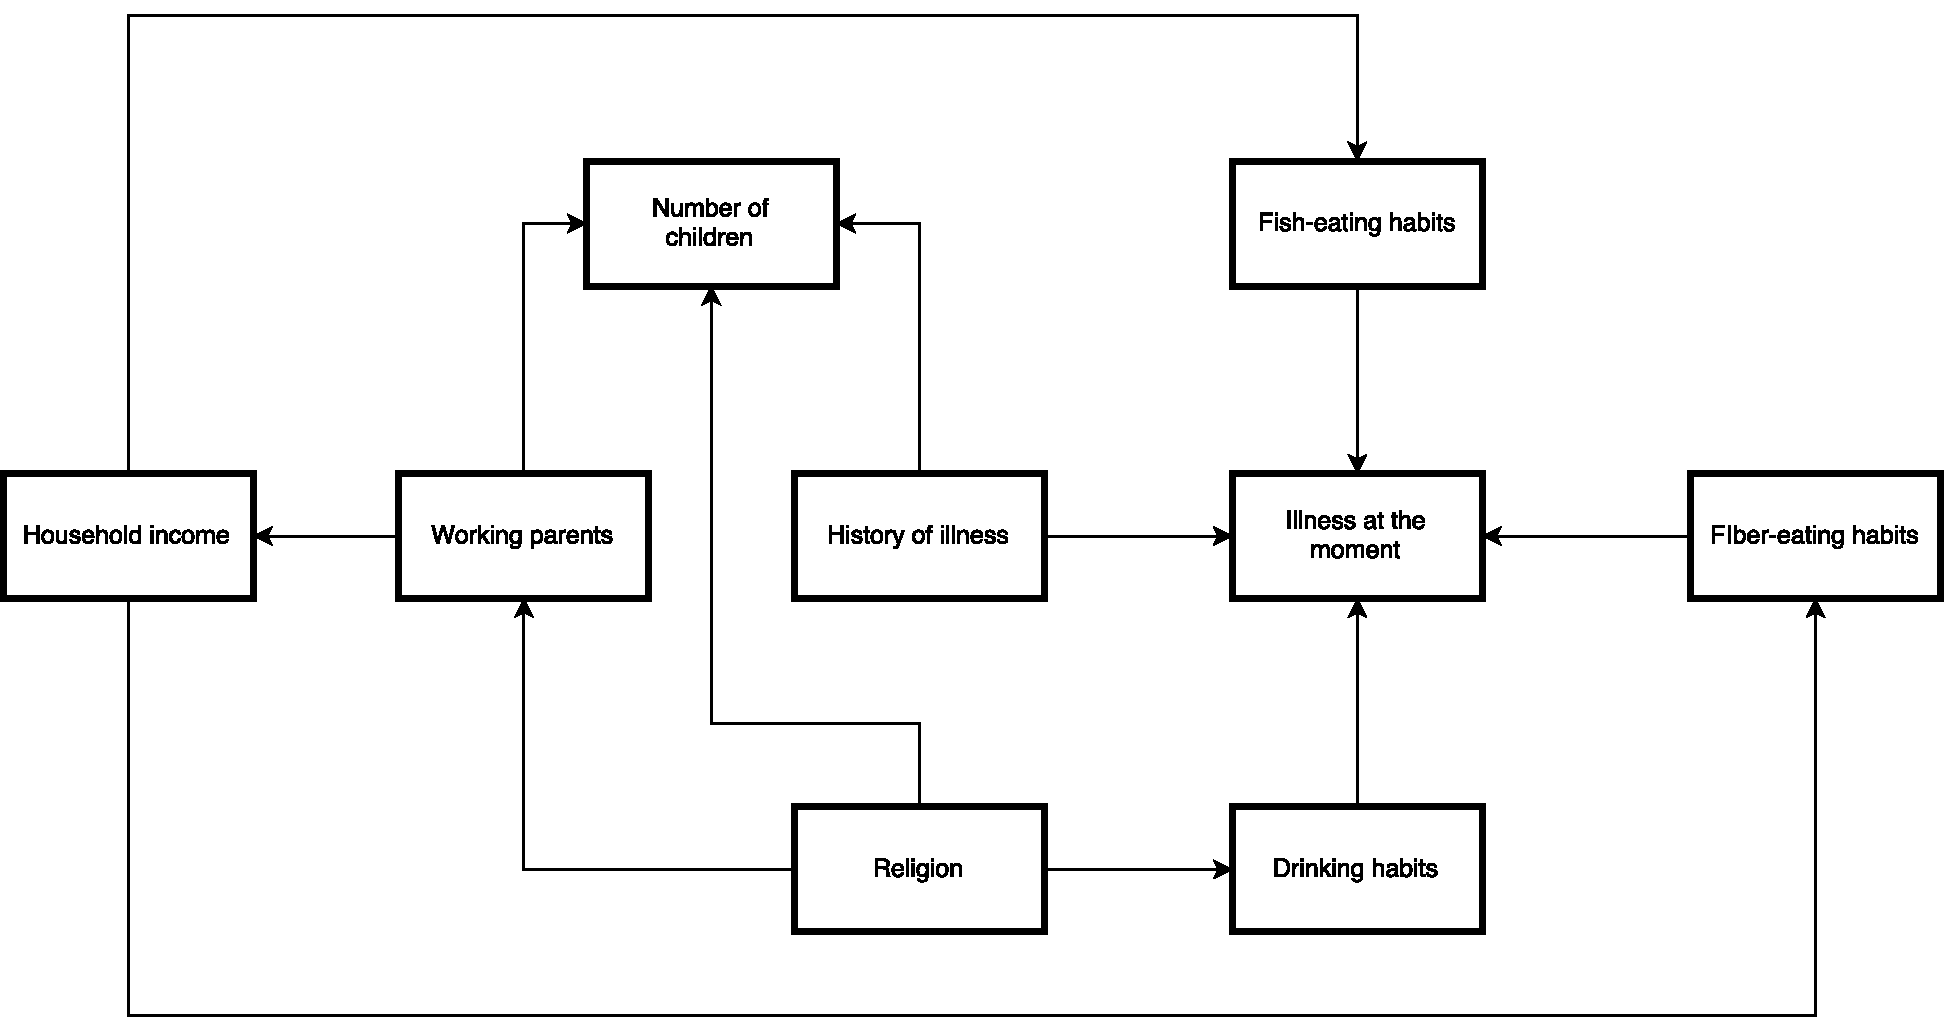
\includegraphics[width=0.75\textwidth]{bayesian_network.pdf}
            \caption{Bayesian network.}
        \end{figure}
        Here is a list of some conditional independencies:
        \begin{itemize}
            \item Religion and history of illness.
            \item Fish-eating habits, fiber-eating habits and drinking habits.
            \item History of illness, fish-eating habits, fiber-eating habits and drinking habits.
            \item Number of children and Illness at the moment.
        \end{itemize}
        I think the results are reasonable, as they model how I perceive the real world. One could argue that there should be drawn more dependencies. If a person eats a lot of fish, they are also probably eating a lot of fibers since they are both healthy. And all the habits can affect the history off illness, which could make one of the parents unable to work. 

    \section{Bayesian Network Application}
        I have choosen to solve this problem using GeNIe, although I have seen the problem before and know that you should always alter your choice.
        \begin{figure}[h!]
            \centering
            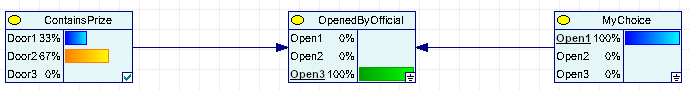
\includegraphics[width=0.75\textwidth]{genie.png}
            \caption{Example probabilites when I choose Door 1 and the official choose door 3.}
        \end{figure}
        \par
        As you can see, the probability for changing door when asked gives you a probability of $\frac{2}{3}$ instead of your original $\frac{1}{3}$.
        \begin{table}[h]
            \centering
            \begin{tabular}{ |c|c|c|c|c|c|c|c|c|c|}
                \hline
                ContainsPrize & \multicolumn{3}{|c|}{Door 1} & \multicolumn{3}{|c|}{Door 2} & \multicolumn{3}{|c|}{Door 3}\\\hline
                MyChoice & 1 & 2 & 3 & 1 & 2 & 3 & 1 & 2 & 3\\\hline
                Open 1 & 0   & 0 & 0 & 0 & 0.5 & 0 & 0 & 1 & 0.5\\
                Open 2 & 0.5 & 0 & 1 & 0 & 0   & 0 & 1 & 0 & 0.5\\
                Open 3 & 0.5 & 1 & 0 & 1 & 0.5 & 1 & 0 & 0 & 0\\\hline
            \end{tabular}
            \caption{The probabilities in OpenedByOfficial.}
        \end{table}



\end{document}
